% 4-2 题 图4_2：质点m绕固定质点m0作圆轨道运动，P为圆周上参考点
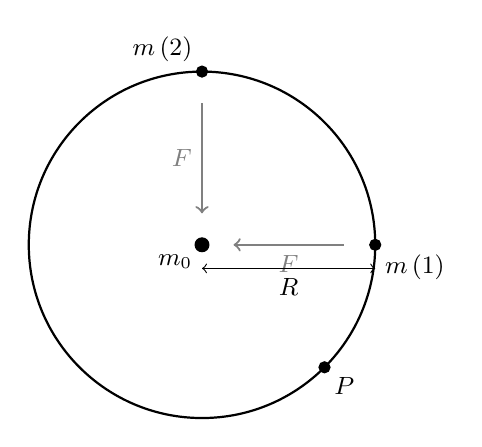
\begin{tikzpicture}[font=\small]
  % 圆轨道
  \draw[thick] (0,0) circle (2.2);
  % 固定质点 m0（在圆心）
  \filldraw (0,0) circle (2.5pt) node[below left] {$m_0$};
  % 质点 m 在点1（右侧）
  \filldraw (2.2,0) circle (2pt) node[below right] {$m$\,(1)};
  % 质点 m 在点2（上方）
  \filldraw (0,2.2) circle (2pt) node[above left] {$m$\,(2)};
  % 参考点P在圆周上（右下角45°位置）
  \coordinate (P) at ({2.2*cos(-45)},{2.2*sin(-45)});
  \filldraw (P) circle (2pt) node[below right] {$P$};
  % 引力方向（从点1指向圆心）
  \draw[->, thick, gray] (1.8,0) -- (0.4,0) node[midway, below] {$F$};
  % 从点2指向圆心
  \draw[->, thick, gray] (0,1.8) -- (0,0.4) node[midway, left] {$F$};
  % 距离R标注（从圆心到点1）
  \draw[<->] (0,-0.3) -- (2.2,-0.3) node[midway, below] {$R$};
\end{tikzpicture}
